\section{Análisis exploratorio de datos}\label{sec:eda}

Se ejecutó el análisis exploratorio sobre \texttt{base\_limia.parquet} con dos objetivos: cada figura se guardó numerada en \texttt{report/figures/} (150 dpi, títulos y ejes en español) y cada figura tiene 2--4 líneas de interpretación escrita. Se generaron 13 figuras y un conjunto de hallazgos numerados H1--H10 que alimentaron las decisiones de ingeniería de características.

\subsection{Distribución del objetivo y desbalance}
\begin{figure}[H]
  \centering
  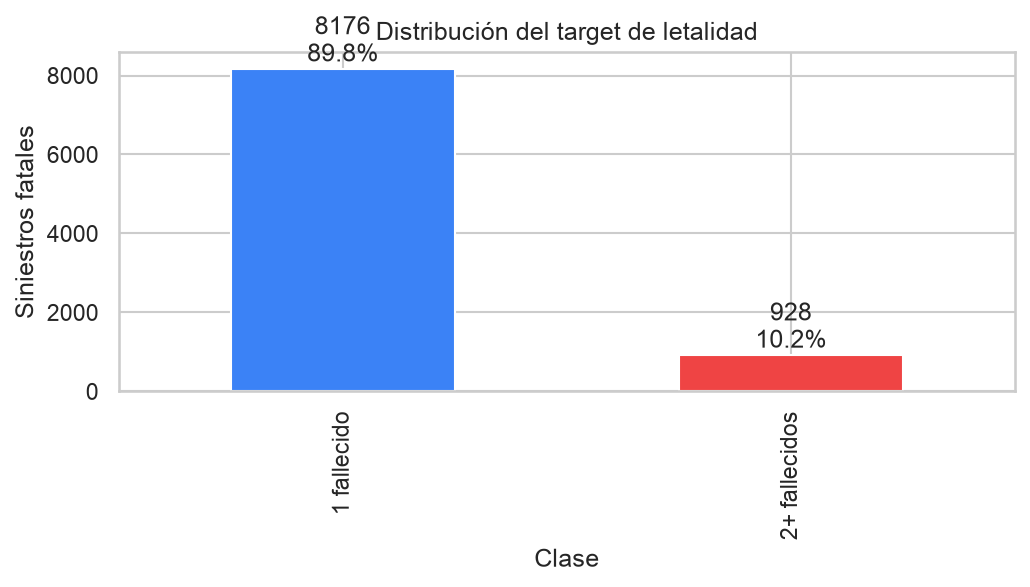
\includegraphics[width=0.7\textwidth]{figures/fig01_target_distribution.png}
  \caption{Distribución del target. La clase mortal representa el 11.7\,\% del dataset limpio, lo que confirma el desbalance y justifica evaluar con F1, \emph{recall} y PR-AUC, no con \emph{accuracy} aislada. (Hallazgo H1.)}
  \label{fig:fig01}
\end{figure}

\subsection{Patrones temporales}
\begin{figure}[H]
  \centering
  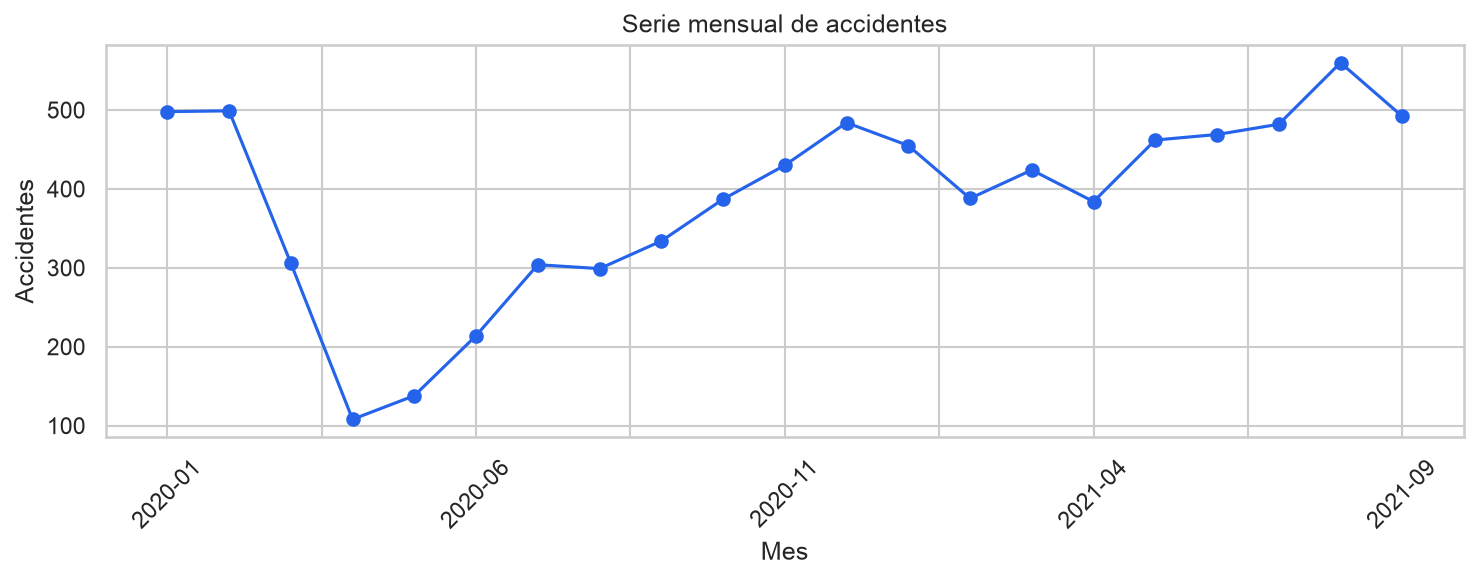
\includegraphics[width=0.8\textwidth]{figures/fig02_monthly_accidents.png}
  \caption{Serie mensual de accidentes. El mes con más accidentes fue agosto 2021 con 560 registros (H2); la frecuencia no es constante, por lo que las variables temporales aportan señal.}
  \label{fig:fig02}
\end{figure}

\begin{figure}[H]
  \centering
  \begin{minipage}{0.49\textwidth}\centering
    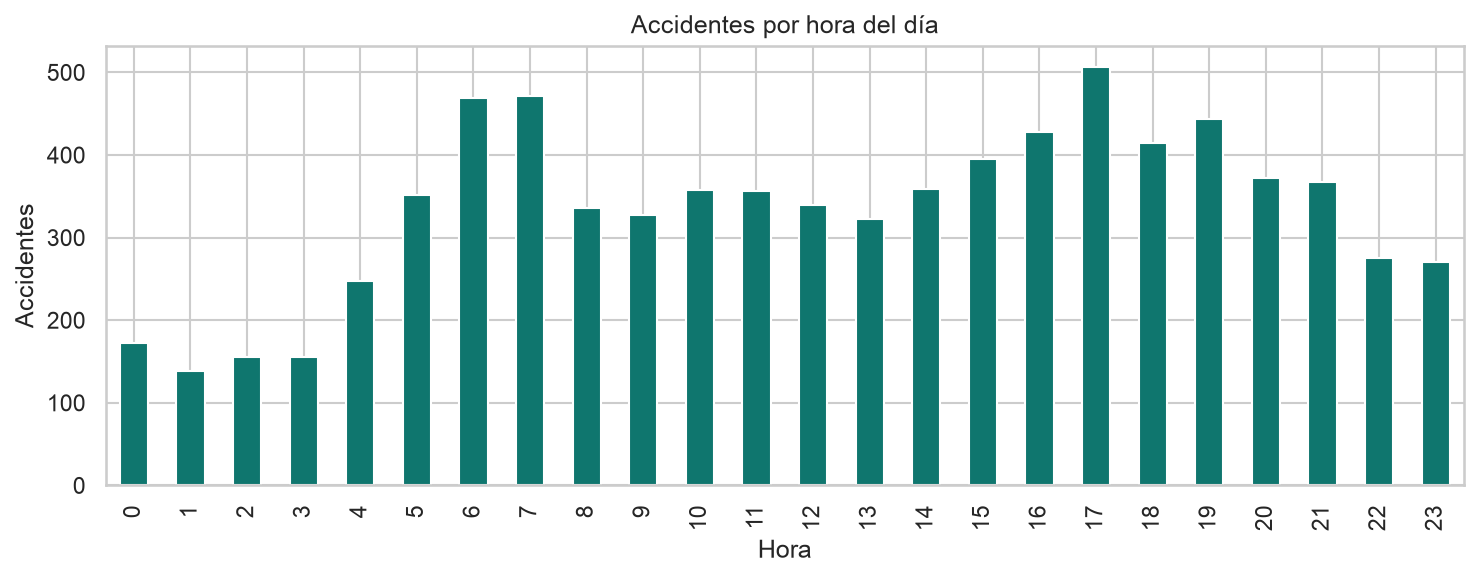
\includegraphics[width=\linewidth]{figures/fig03_accidents_by_hour.png}
    \caption{Accidentes por hora del día. La hora con más accidentes fue 17:00 (H3).}
    \label{fig:fig03}
  \end{minipage}\hfill
  \begin{minipage}{0.49\textwidth}\centering
    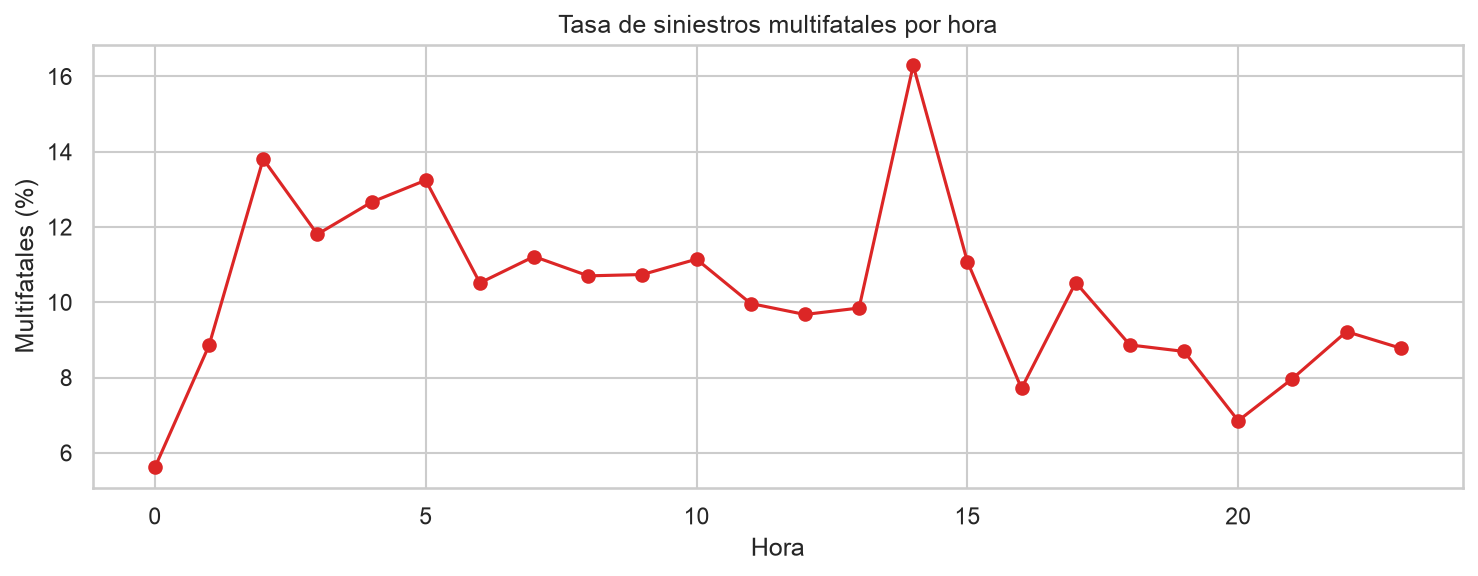
\includegraphics[width=\linewidth]{figures/fig04_mortality_rate_by_hour.png}
    \caption{Tasa de mortalidad por hora. La mayor tasa (18.8\,\%) aparece a las 01:00 (H3): volumen y severidad no son lo mismo.}
    \label{fig:fig04}
  \end{minipage}
\end{figure}

\begin{figure}[H]
  \centering
  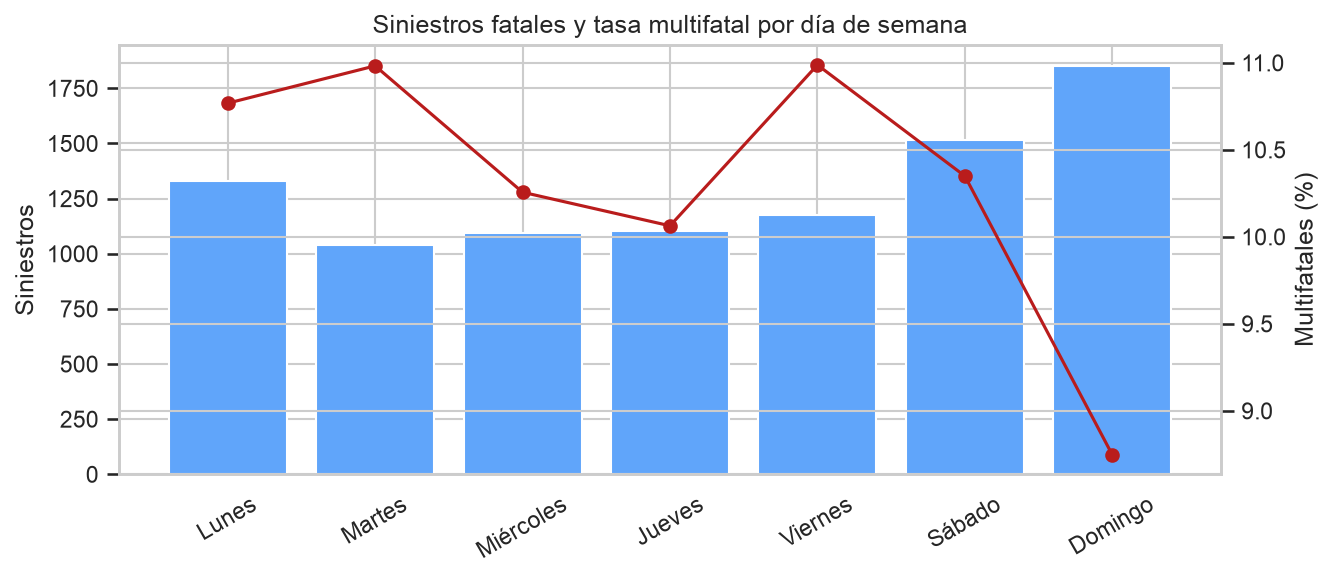
\includegraphics[width=0.8\textwidth]{figures/fig05_weekday_accidents_mortality.png}
  \caption{Accidentes y tasa de mortalidad por día de semana. Cantidad y severidad deben leerse juntas (H4). Esto respalda incluir \texttt{dia\_semana} y \texttt{fin\_de\_semana} como señales distintas.}
  \label{fig:fig05}
\end{figure}

\subsection{Modalidad: el hallazgo más fuerte}
\begin{figure}[H]
  \centering
  \begin{minipage}{0.49\textwidth}\centering
    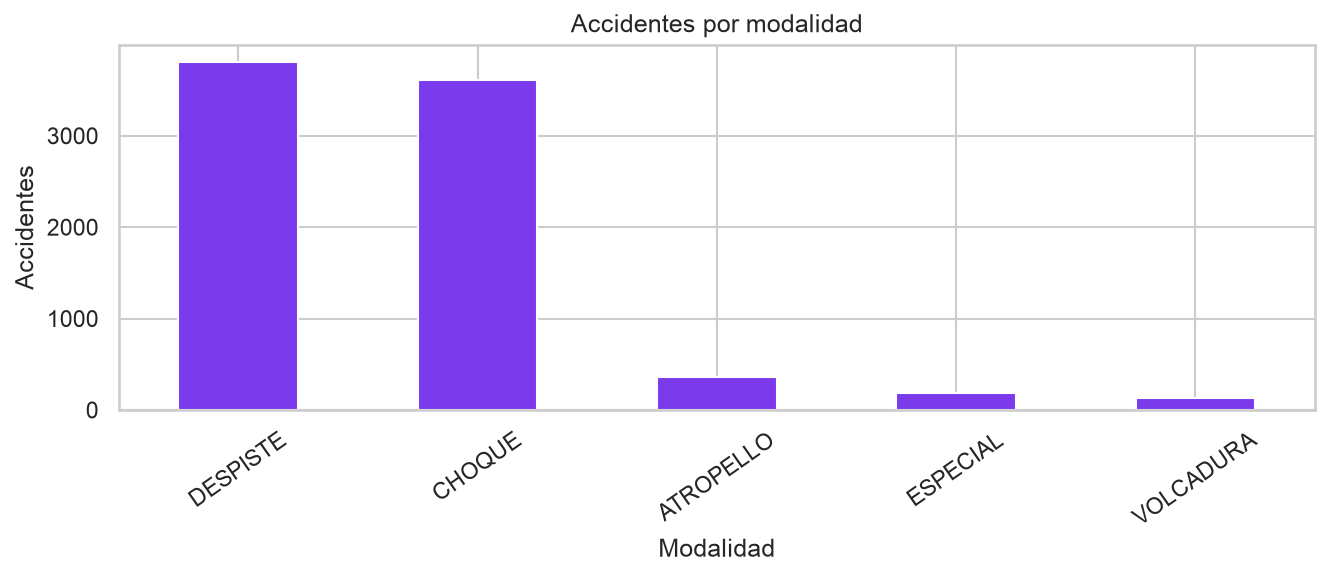
\includegraphics[width=\linewidth]{figures/fig06_accidents_by_modality.png}
    \caption{Cantidad de accidentes por modalidad. La más frecuente fue DESPISTE con 3\,806 casos (H5).}
    \label{fig:fig06}
  \end{minipage}\hfill
  \begin{minipage}{0.49\textwidth}\centering
    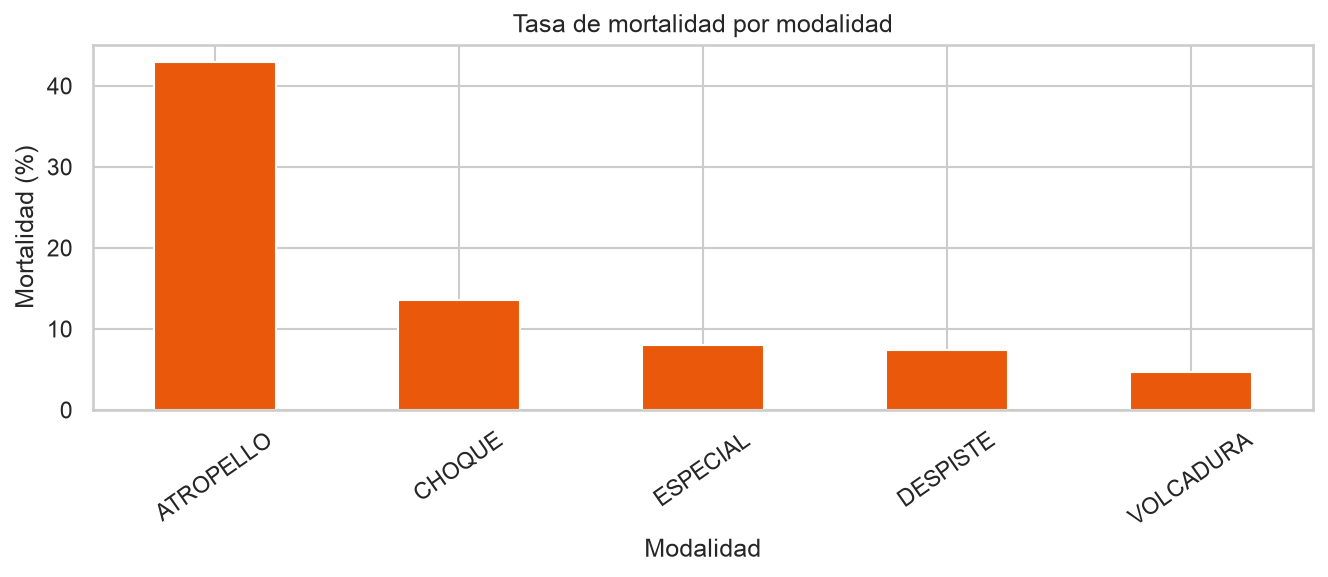
\includegraphics[width=\linewidth]{figures/fig07_mortality_by_modality.png}
    \caption{Tasa de mortalidad por modalidad. ATROPELLO presenta 42.9\,\% (H5), el hallazgo más fuerte del proyecto; anticipa que MODALIDAD será una característica dominante.}
    \label{fig:fig07}
  \end{minipage}
\end{figure}

\subsection{Análisis territorial}
\begin{figure}[H]
  \centering
  \begin{minipage}{0.49\textwidth}\centering
    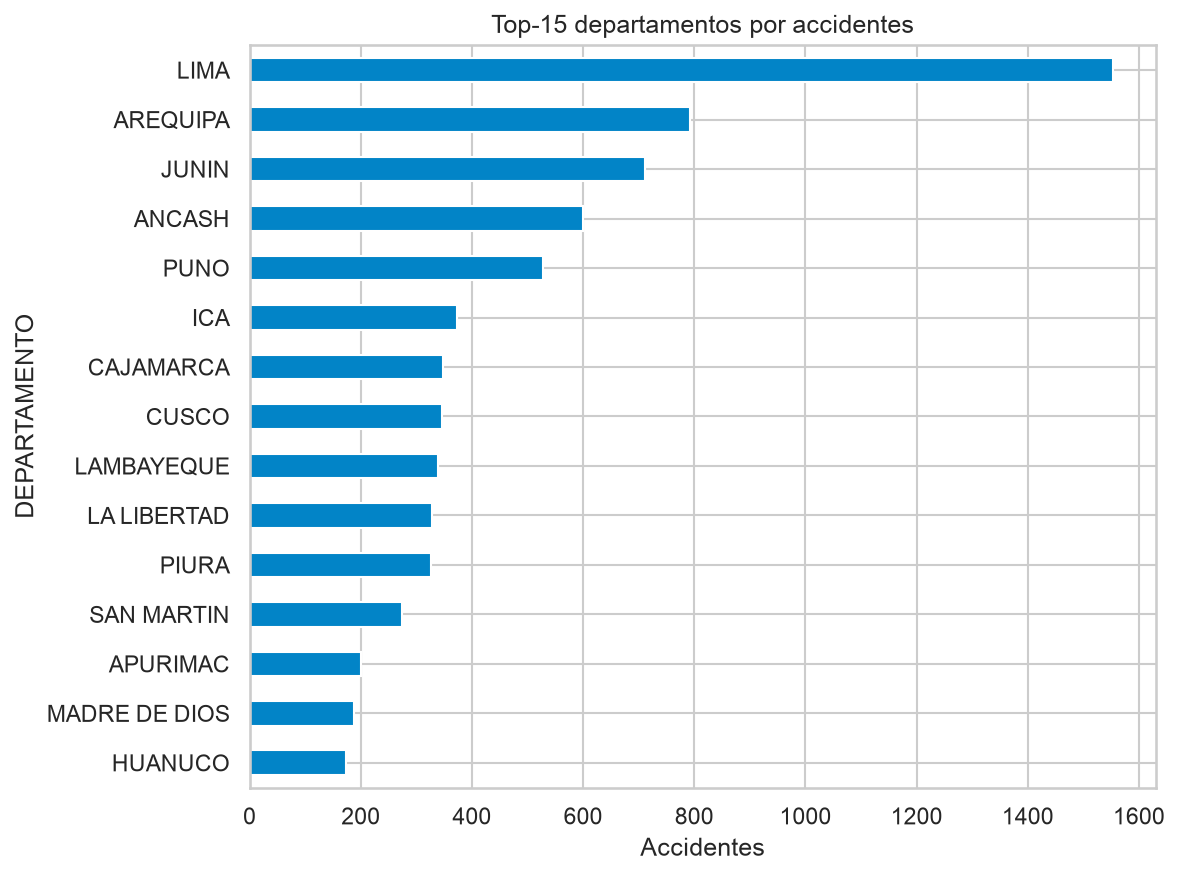
\includegraphics[width=\linewidth]{figures/fig08_top_departments_accidents.png}
    \caption{Top-15 departamentos por número de accidentes. LIMA concentra 1\,553 (H6).}
    \label{fig:fig08}
  \end{minipage}\hfill
  \begin{minipage}{0.49\textwidth}\centering
    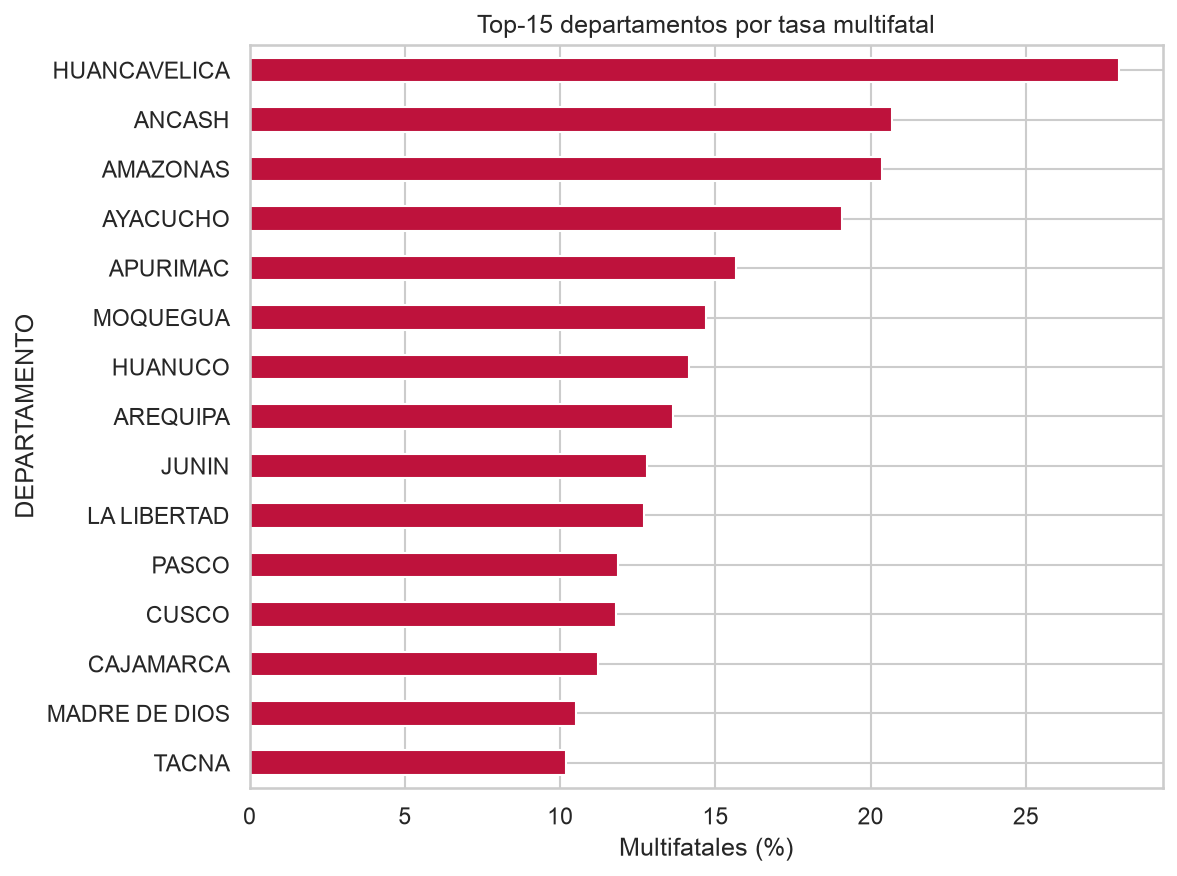
\includegraphics[width=\linewidth]{figures/fig09_top_departments_mortality.png}
    \caption{Top-15 departamentos por tasa de mortalidad. LA LIBERTAD lidera con 22.3\,\% entre departamentos con al menos 30 casos (H6). El ranking por volumen no equivale al ranking por severidad.}
    \label{fig:fig09}
  \end{minipage}
\end{figure}

\subsection{Vías y tramos}
\begin{figure}[H]
  \centering
  \begin{minipage}{0.49\textwidth}\centering
    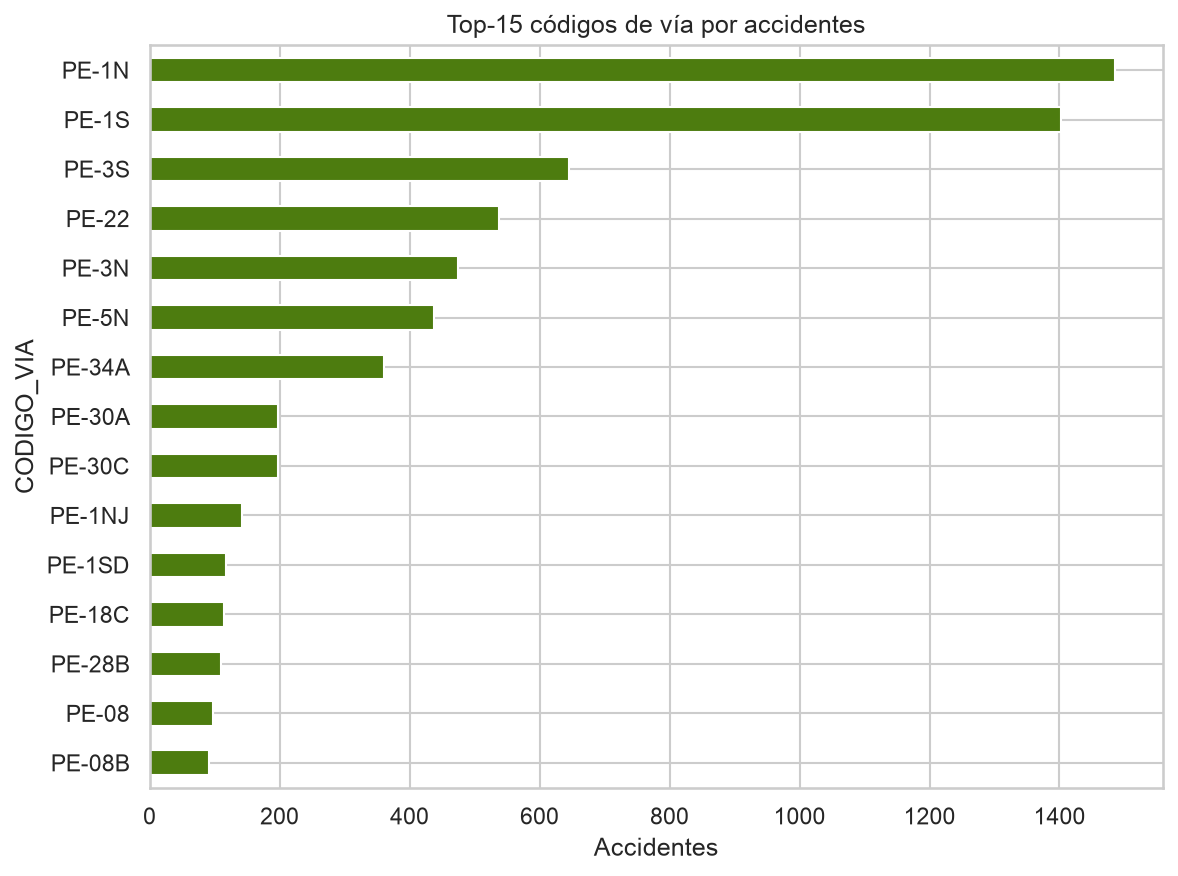
\includegraphics[width=\linewidth]{figures/fig10_top_roads_accidents.png}
    \caption{Top-15 códigos de vía por número de accidentes. La vía PE-1N encabeza con 1\,485 casos (H7).}
    \label{fig:fig10}
  \end{minipage}\hfill
  \begin{minipage}{0.49\textwidth}\centering
    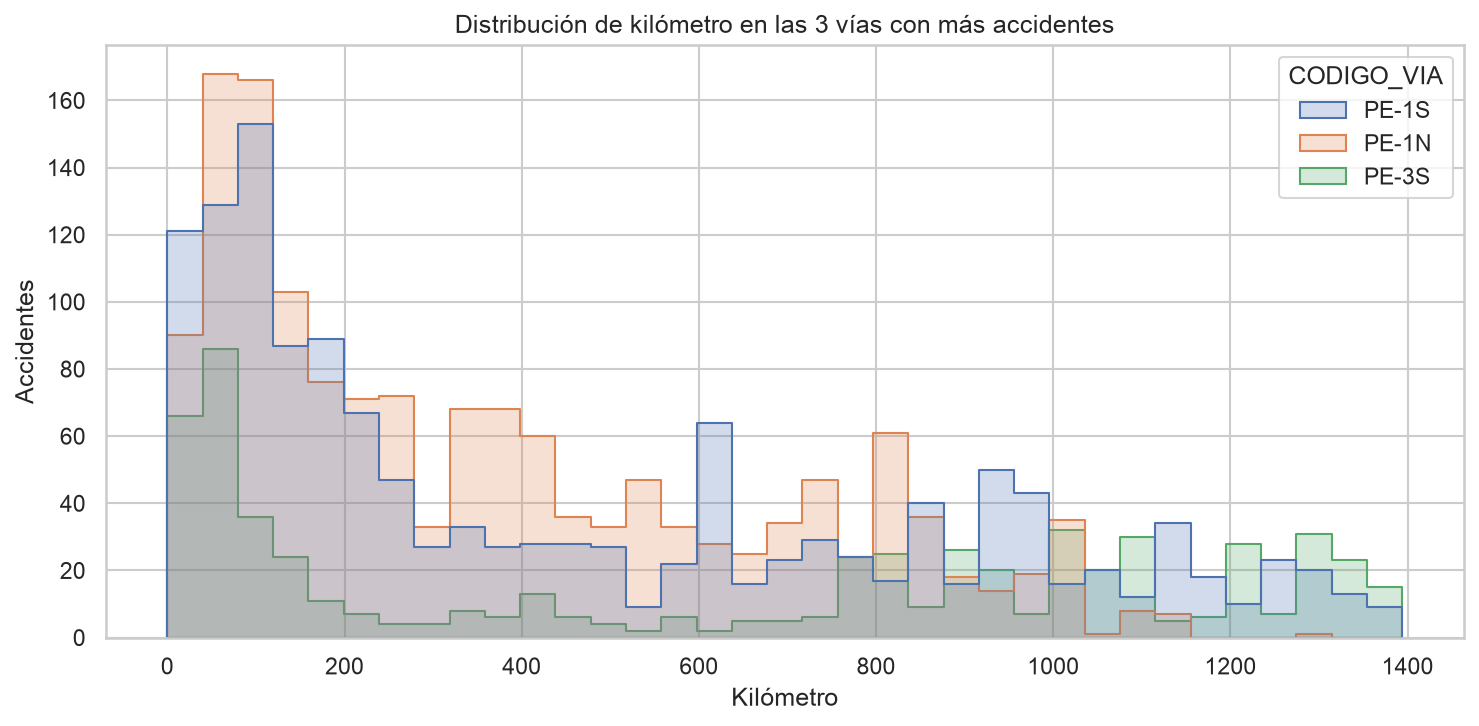
\includegraphics[width=\linewidth]{figures/fig11_kilometer_distribution_top_roads.png}
    \caption{Distribución de \texttt{KILOMETRO} en las tres vías con más accidentes. La concentración por tramos (H8) justifica conservar \texttt{KILOMETRO} como variable numérica con imputación controlada.}
    \label{fig:fig11}
  \end{minipage}
\end{figure}

\subsection{Patrones combinados y calidad de datos}
\begin{figure}[H]
  \centering
  \begin{minipage}{0.49\textwidth}\centering
    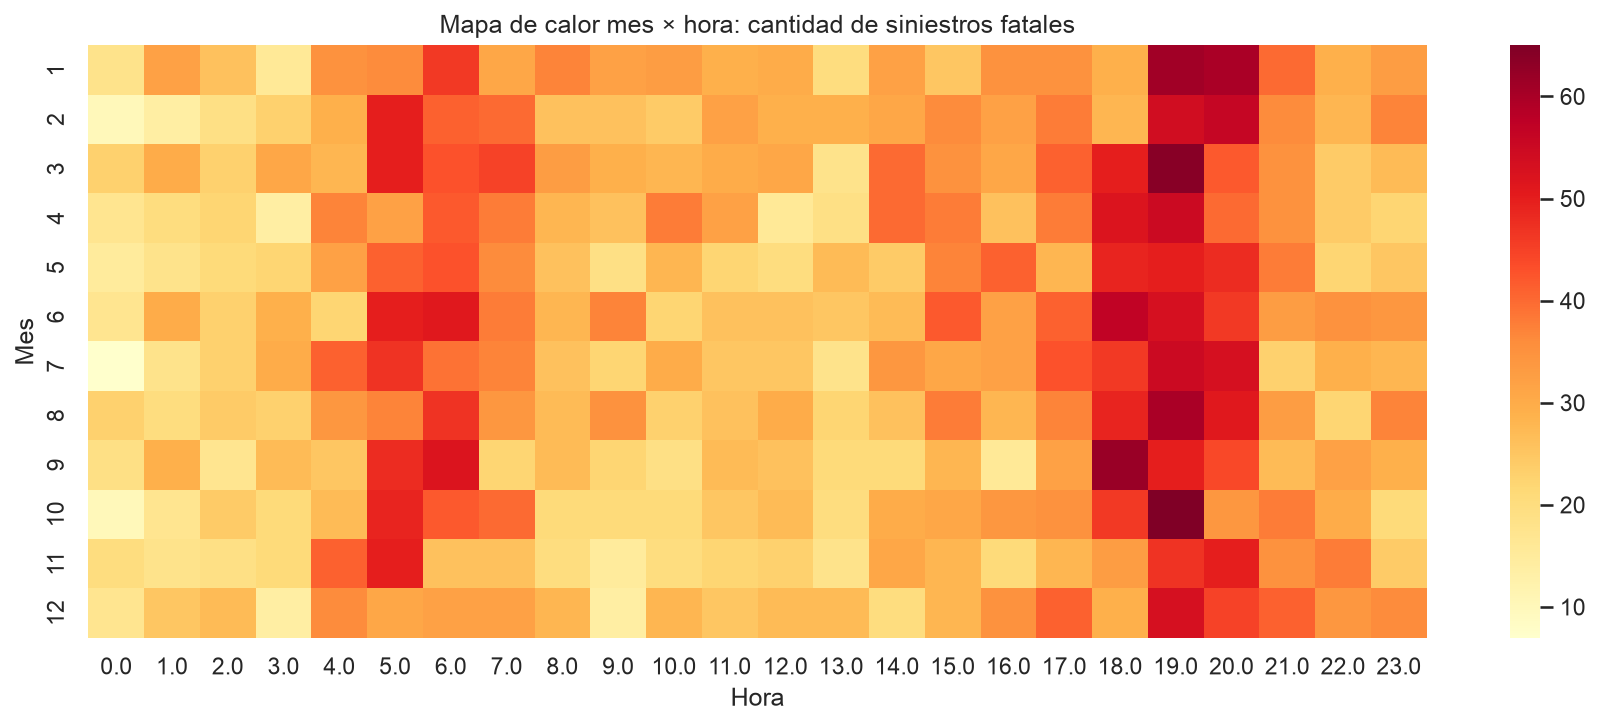
\includegraphics[width=\linewidth]{figures/fig12_month_hour_heatmap.png}
    \caption{Mapa de calor mes $\times$ hora. Los patrones combinados (H9) prueban que no basta con fecha u hora cruda: se requieren derivadas cíclicas y de franja.}
    \label{fig:fig12}
  \end{minipage}\hfill
  \begin{minipage}{0.49\textwidth}\centering
    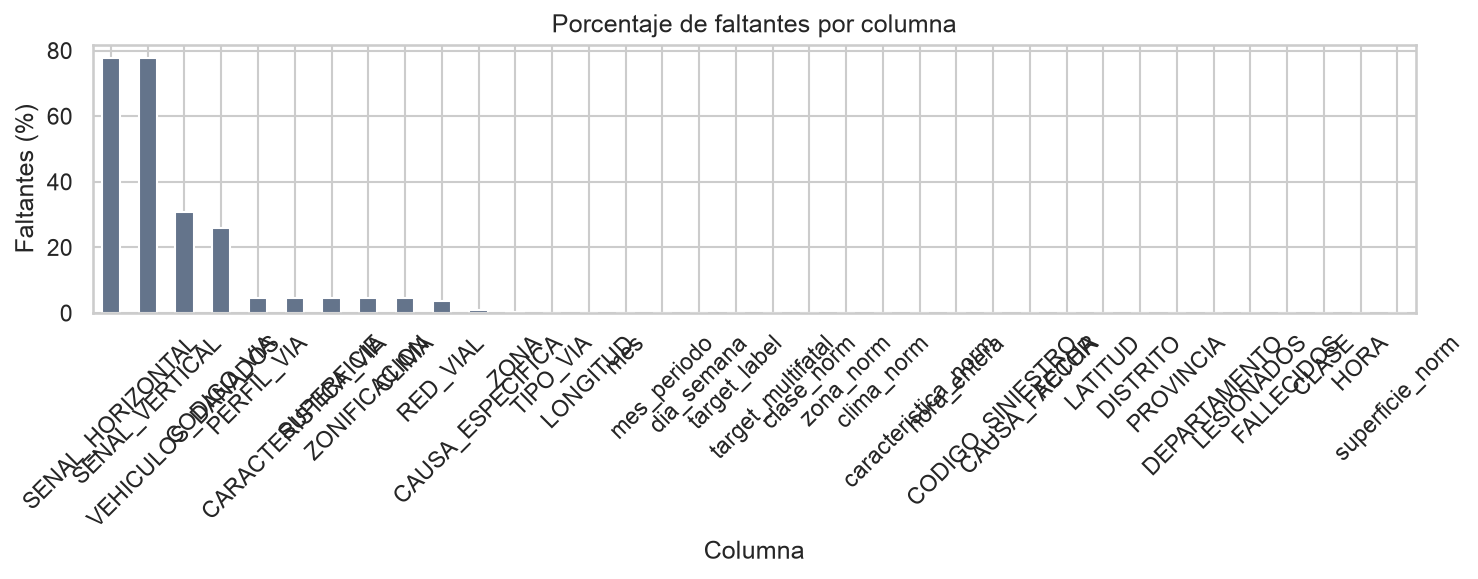
\includegraphics[width=\linewidth]{figures/fig13_missing_values.png}
    \caption{Matriz de porcentaje de faltantes por columna. La mayor magnitud es \texttt{HORA} con 1.1\,\% (H10): suficiente para imputaciones simples con \emph{flags}.}
    \label{fig:fig13}
  \end{minipage}
\end{figure}

\subsection{Hallazgos H1--H10}
Se redactaron diez hallazgos en prosa, cada uno con referencia a su figura. Los más relevantes para el modelado:
\begin{itemize}
  \item \textbf{H1}: la clase mortal representa 11.7\,\% del dataset limpio (figura~\ref{fig:fig01}), confirma desbalance y justifica las métricas.
  \item \textbf{H3}: la hora con más accidentes (17:00) no coincide con la de mayor tasa de mortalidad (01:00, 18.8\,\%) (figuras~\ref{fig:fig03} y \ref{fig:fig04}). Volumen y severidad son dimensiones distintas.
  \item \textbf{H5}: DESPISTE es la modalidad más frecuente, pero ATROPELLO tiene la mayor tasa de mortalidad (42.9\,\%) (figuras~\ref{fig:fig06} y \ref{fig:fig07}). MODALIDAD será una característica dominante.
  \item \textbf{H6}: LIMA concentra la mayor cantidad de accidentes, pero LA LIBERTAD lidera la tasa de mortalidad (figuras~\ref{fig:fig08} y \ref{fig:fig09}).
  \item \textbf{H9}: el mapa mes $\times$ hora evidencia patrones combinados (figura~\ref{fig:fig12}), justificando derivadas cíclicas y de franja.
\end{itemize}